\chapter{Fast Generalized Distillation for Semi-supervised Domain Adaptation}
\section{Introduction}

\section{Previous Work}\label{sec:aaai:work}
As we use GD to solve SDA problem, we introduce related work in both GD and SDA areas.

In SDA, previous work tried to utilize the unlabeled data to improve the performance.  \cite{yao2015semi} introduced a framework named Semi-supervised Domain Adaptation with Subspace Learning (SDASL) to correct data distribution mismatch and leverage unlabeled data. \cite{Donahue_2013_CVPR} proposed a framework for adapting classifiers by ``borrowing" the source data to the target domain using a combination of available labeled and unlabeled examples. \cite{daume2010frustratingly} show that augmenting the feature space of the data can compensate the domain shift.
\cite{duan2009domain} proposed a method using the unlabeled data to measure the mismatch between different domains based on the maximum mean discrepancy. %\cite{reddi2015doubly} proposed 

There are also many studies related to GD for computer vision tasks. \cite{Sharmanska_2013_ICCV} proposed a Rank Transfer method that uses attributes, annotator
rationales, object bounding boxes, and textual descriptions as the privileged information for object recognition. \cite{Motiian_2016_CVPR} proposed {the information bottleneck method with privileged information (IBPI)} that leverage the auxiliary information such as supplemental visual features, bounding box annotations and 3D skeleton tracking data to improve visual recognition performance. \cite{Tzeng_2015_ICCV} proposed a CNN architecture for domain adaptation to leverage the knowledge from limited or no labeled data using the soft label. \cite{urban2016deep} used a small shallow net to mimick the output of a large deep net while using layer-wised distillation with $\ell_2$ loss of the outputs of the student and teacher net. Similarly, \cite{luo2016face} used $\ell_2$ loss to train a compressed student model from the teacher model for face recognition. 

Compared to previous work on SDA, our method only requires the output of the source models, which is more effective when the size of the source domain is relatively large and the source model is well-trained. Compared to other work in GD, our method GDSDA-SVM can effectively estimate the imitation parameter while previous work was limited to using either a brutal force search or domain knowledge.

\section{Generalized Distillation for Semi-supervised Domain Adaptation}\label{sec:aaai:gdda}
As previously mentioned, GDSDA is a paradigm using generalized distillation for semi-supervised domain adaptation. In this section, we first give a brief review of generalized distillation. Then we show the process of GDSDA and demonstrate the reason why GDSDA can work for the SDA problem. Finally, we show the importance of the imitation parameter. 
\begin{figure}\label{fig:gd}
	\centering
	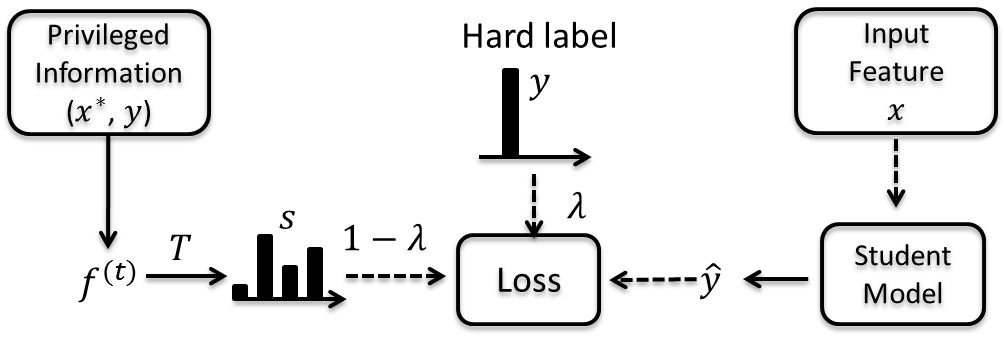
\includegraphics[scale=.6]{aaai/figure/GD.png}
	\caption{Illustration of Generalized Distillation training process.}
\end{figure}
\subsection{An overview of Generalized Distillation and GDSDA}
\textit{Distillation} \cite{hinton2015distilling} and \textit{Learning Using Privileged Information} (LUPI) \cite{vapnik2015learning} are two paradigms that enable machines to learn from other machines. Both methods address the problem of how to build a student model that can learn from the advanced teacher models. Recently, \cite{lopez2015unifying} proposed a framework called \textit{generalized distillation} that unifies both methods and show that it can be applied in many scenarios.

In GD, the training data can be represented as a collection of the triples:
\[\{\left(x_1,x_1^*,y_1\right),\left(x_2,x_2^*,y_2\right) \dots \left(x_n,x_n^*,y_n\right)\}\]
$x^*$ is the privileged information for data $x$, which is only available in the training set and $y$ is the corresponding label. Therefore, the goal of GD is to train a model, called student model with the guidance of the privileged information to predict the unseen example pair $(x,y)$.

The process of generalized distillation is as follows: in step 1, a teacher model ${f}^{(t)}$ is trained using the input-output pairs $\{x^*_i,y_i\}_{i=1}^n$. In step 2, use ${f}^{(t)}$ to generate the soft label $s_i$ for each training example $x_i$ using the softmax function $\sigma$:
\begin{equation}\label{eq:softmax_T}
s_i=\sigma(f^{(t)}(x_i)/T)
\end{equation}
where $T$ is a parameter called temperature to control the smoothness of the soft label. In step 3, learn the student ${f}^{(s)}$ from the pairs $\{\left(x_i,y_i\right),\left(x_i,s_i\right)\}_{i=1}^n$ using:
\begin{equation}\label{eq:distill}
\begin{aligned}
f^{(s)}=&\underset{f^{(s)} \in \mathcal{F}^{(s)}}{\arg \min}\frac{1}{n}\sum_{i=1}^{n}\bigg[\lambda\ell\left(y_i,\sigma(f^{(s)}(x_i))\right)
+(1-\lambda)\ell\left(s_i,\sigma(f^{(s)}(x_i))\right)\bigg]\\
\end{aligned}
\end{equation}
Here, $\ell(\cdot,\cdot)$ is the loss function and $\lambda$ is the imitation parameter to balance the importance between the hard label $y_i$ and the soft label $s_i$.

GD can be used in many scenarios such as multi-task learning, semi-supervised learning, and reinforcement learning. In domain adaptation, when we consider the source model as the teacher and the predictions of the target data given by the source models as the privileged information,
GD can be naturally applied to SDA. This leads to \textit{Generalized Distillation Semi-supervised Domain Adaptation} (\textbf{GDSDA}). Moreover, in GDSDA, we also consider the multi-source scenario and extend the GD paradigm to fit this scenario. To be consistent with other work of domain adaptation, we use the \textit{source model} and the \textit{target model} to denote the teacher model and the student model.
\begin{figure}
	\centering
	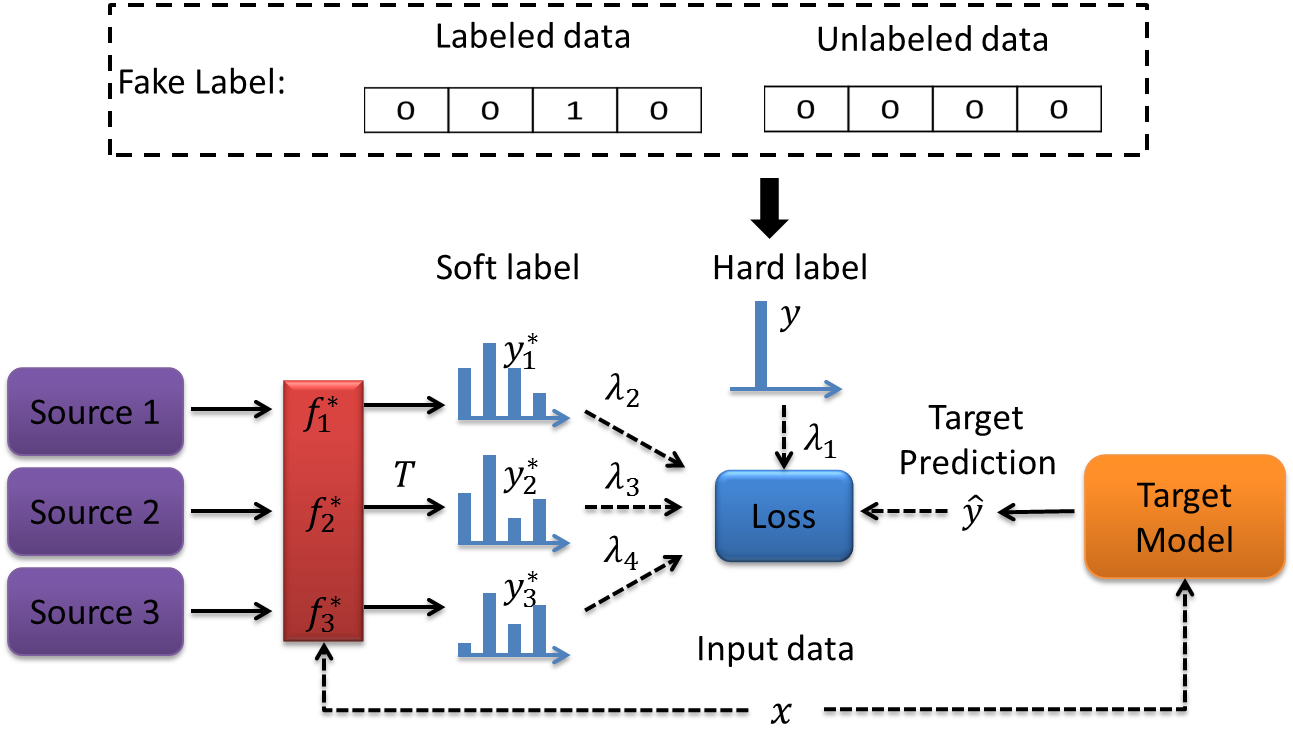
\includegraphics[scale=.5]{aaai/figure/multi-GDDA.png}
	\caption{Illustration of GDSDA training process and our ``fake label" strategy.}\label{fig:GDSDA}
\end{figure}

Technically, when we apply GD to SDA, according to Eq. \eqref{eq:distill}, each example is assigned with a hard label $y$ (true label) and a soft label $s$ (class probabilities from the teacher). However, in SDA, we are not able to obtain the hard labels of the unlabeled data. Here we follow the GD work\cite{lopez2015unifying} and use the ``fake label" strategy to label the unlabeled data: for the labeled examples, we use \textit{one-hot} strategy to encode their labels while using all 0s as the label of the unlabeled examples (see Fig \ref{fig:GDSDA}). Thus, each example in the target domain is assigned with a label. It is arguable that the ``fake label" strategy would introduce extra noise and degrade the performance. However, we will show in our experiment that this noise can be well controlled by setting a proper value to the imitation parameter and we can still achieve improved performance (See the single source experiment).

Suppose we have $M-1$ source domains denoted as $D_s^{(j)}=\{X^{(j)},Y^{(j)}\}_{j=1}^{M-1}$ and the target domain $D_t=\{X,Y\}$ encoded with the ``fake label" strategy. The process of GDSDA is as follows:
\begin{enumerate}
	\item Train the source models $f^*_j$ for each of the $M-1$ domains with $\{X^{(j)},Y^{(j)}\}$.
	\item For each of the training example $x_i$ in the target domain, generate the corresponding soft label $y^*_{ij}$ with each of the source model $f^*_j$ and the temperature $T>0$.
	\item Learn the target model $f_t$ using the $(M+1)$-tuples $\{x_i,y_i,y^*_{i1},\dots,y^*_{i(M-1)}\}_{i=1}^L$ with the imitation parameters $\{\lambda_i\}^M_{i=1}$ using \eqref{eq:GDDA_abs}:
\end{enumerate} 
\begin{equation}\label{eq:GDDA_abs}
\begin{aligned}
f_t(\lambda)=&\underset{f_t \in \mathcal{F}}{\arg \min}\frac{1}{L}\sum_{i=1}^{L}\bigg[\lambda_1\ell\left(y_i,f_t(x_i)\right)+\sum_{j=1}^{M-1}\lambda_{j+1}\ell\left(y^*_{ij},f_t(x_i)\right)\bigg]\\
\text{s.t.} & \qquad \sum_i\lambda_i=1
\end{aligned}
\end{equation}
Compared to other studies on SDA where each example of the source domain was used, by either re-weighting \cite{Donahue_2013_CVPR,duan2012visual} or augmentation \cite{daume2010frustratingly}, GDSDA only requires the trained model from the source domain to generate the soft labels. Considering that it is more convenient to access the source model than each of the examples of the source domain, GDSDA can be more useful than those previous methods. For example, if we want to use ImageNet \cite{imagenet_cvpr09} as the source domain, it is almost impossible to access each of the millions of examples while there are many well trained models publicly available online that can be used for GDSDA. Also, GDSDA is able to handle the multi-class scenario while previous methods, such as SHFA\cite{duan2012learning} only solved the binary classification problem of SDA. Moreover, GDSDA is compatible with any type of source model that is able to output the soft label (i.e., the class probabilities).

\subsection{Why does GDSDA work}
In this section, we demonstrate the scenarios where GDSDA can work. Before we provide our analysis, we first introduce two basic assumptions for GDSDA: the \textit{assumption of distillation} and the \textit{assumption of the source model}.

\textbf{Assumption of Distillation:} The capacity (or VC dimension) of the target model $f_t$ is smaller than the capacity of source model $f^*$. This assumption is inherited from distillation \cite{lopez2015unifying}.
\textbf{Assumption of the source model:} The source model $f^*$ should work better than a target model $f'_t$ trained only with the hard labels. This assumption is common, especially in SDA where the labeled examples are often too few to build a good target model. For example, when we only have one labeled example from each class in the target training set, it is reasonable to assume that the source model trained from another domain can perform better than the model trained only with the target training data on the target task. Based on these two assumptions, we will show that GDSDA can effectively leverage the source model and transfer the knowledge between different domains under the SDA setting.

According to the ERM principle\cite{vapnik1999overview}, a simple model has better generalization ability than the complex one, if they both have the same training error.
As long as the target model $f_t$ can achieve similar training error to that of the source model $f^*$ on the target domain, considering the fact that the VC dimension of $f_t$ is smaller than $f^*$, we can expect that the target model has better generalization ability. This process can be achieved by letting the target model mimick the output of the source model on the training data.
It is worthy to notice that in this process, the target model only has to mimick the output of the source model (soft label) without considering the hard labels of the examples. In another word, GDSDA provide an effective way to utilize the unlabeled data.

Arguably, because of the domain shift, the source model is biased towards the source domain when we apply it to the target task. However, as suggested in \cite{hinton2015distilling}, we can use labeled data from the target domain to compensate for the domain shift and achieve a better performance on the target task with Eq. \eqref{eq:GDDA_abs}. Specifically, we use the imitation parameter $\lambda$ to control the relative importance between the soft label and the hard label, which in turn reflects the similarity between the source and target tasks. 
For example, in Figure \ref{fig:GDSDA}, when we set $\lambda_2=0$, we actually ignore the knowledge from source domain 1.
As a result, GDSDA can compensate for the domain shift under the setting of SDA (for more details, please see the experiment section).

\subsection{Key parameter: the imitation parameter}\label{sec:aaai:key}
From the above analysis, we can see that GDSDA can effectively transfer the knowledge from the source to the target domain. In this section, we demonstrate that the imitation parameter can greatly affect the performance of the target model.

In GDSDA, we must decide the values of 2 parameters, the temperature $T$ and the imitation parameter $\lambda$. The temperature $T$ controls the smoothness of the soft label and the imitation parameter $\lambda$ controls how much knowledge can be transferred from the source model. Previous work has addressed the importance of knowledge control in domain adaptation \cite{duan2012learning,duan2012visual}. Without carefully controlling the amount of knowledge transferred from the source domain, the target model may suffer from degraded performance or even negative transfer \cite{pan2010survey}.
How to choose the imitation parameter is crucial for GDSDA. In previous work, however, the imitation parameter was determined by either a brute force search \cite{lopez2015unifying} or background knowledge \cite{Tzeng_2015_ICCV}. Meanwhile, in real applications, it is common that  multiple source domains can be exploited. As suggested by \cite{tommasi2014learning}, learning from multiple related sources simultaneously can significantly improve the performance of the target model. However, these previous methods become more difficult to apply when there are multiple sources and imitation parameters to be determined.
For these reasons, it is ideal to find an approach that can determine the imitation parameter automatically.

\section{GDSDA-SVM}\label{sec:aaai:svm}
As previously mentioned, it is important to find an approach that can effectively determine the imitation parameter. In this section, we propose our method GDSDA-SVM which uses SVM as the base classifier and can effectively estimate the imitation parameter by minimizing the cross-validation error on the target domain.
\subsection{Distillation with multiple sources}
As suggested in \cite{vapnik2015learning}, the optimal imitation parameter should be the one that can minimize the training error on the target domain. Based on that, we propose our method GDSDA-SVM which can effectively estimate the imitation parameter.

Instead of using hinge loss in our GDSDA-SVM, we use Mean Squared Error (MSE) as our loss function for the following two reasons: (1) several recently studies \cite{ba2014deep,luo2016face,romero2014fitnets,urban2016deep} show that MSE is also an efficient measurement for the target model to mimick the output of the source model. (2) MSE can provide a closed form cross-validation error estimation which allows us to estimate the imitation parameter effectively. 

Suppose we have $L$ examples $\{\textbf{x}_j,\textbf{y}_j\}_{j=1}^L$ from $N$ classes in the target domain where $X\in R^{L\times d}, Y\in R^{L\times N}$. Meanwhile, there are $M-1$ source (teacher) models providing the soft labels $Y^*=\{\textbf{y}^*_{ij}|j=1,...,L;i=1,...,M-1\}$ for each of the $L$ examples.
For simplicity, we concatenate the hard label $Y$ and soft label $Y^*$ into a new label matrix $S$, where:
\[S=[Y;Y^*]=[S_1;...;S_M]; S_i \in R^{L \times N}\]
To solve this $N$-class classification problem, we adopt the One-vs-All strategy to build $N$ binary SVMs.
To build the $n$th binary SVM, we have to solve the following optimization problem: 
\begin{equation}\label{eq:multi-distill}
\begin{aligned}
\underset{w_n}{\min} \qquad & \frac{1}{2}{|| \textbf{w}_n ||^2} + C\sum_{j}{e_{jn}^2} \quad\\
s.t. \qquad& e_{jn} = \sum_i\lambda_iS_{ijn} - \textbf{w}_n\textbf{x}_j%;\sum_i\lambda_i=1;\\
%& \sum_i\lambda_i=1; \lambda_i \in [0,1]; i\in M;  j\in L\\
\end{aligned}  
\end{equation}
We use the KKT theorem \cite{cristianini2000introduction} and add dual sets of variables to the Lagrangian of the optimization problem:
\begin{equation}
\begin{aligned}
\mathcal{L}=&\frac{1}{2}{|| \textbf{w}_n ||^2} + C\sum_{j} {e_{jn}^2}\\
&+\sum_{j}\eta_{jn}\left(\sum_i\lambda_iS_{ijn} - \textbf{w}_n\textbf{x}_j-e_{jn}\right)%+\beta^{(n)}\left(\sum_i\lambda_i-1\right)
\end{aligned}
\end{equation}
To find the saddle point, 
\begin{equation}
\begin{aligned}
\frac{{\partial \mathcal{L}}}{{\partial \textbf{w}_n}}& =0 \rightarrow \textbf{w}_n = \sum_{j}\eta_{jn} {\textbf{x}_j}; &
\frac{{\partial \mathcal{L}}}{{\partial {e_{jn}}}} & =0 \rightarrow \eta_{jn} = 2C {e_{jn}}\\
\end{aligned}
\end{equation}
For each example $\textbf{x}_j$ and its constraint of label $S_{ijn}$, we have $e_{jn}  + \textbf{w}_n\textbf{x}_j= \sum_i\lambda_iS_{ijn}$. Replacing $\textbf{w}_n$ and $e_{jn}$,  we have:
\begin{equation}
\begin{aligned}
\sum_j\eta_{jn}\textbf{x}_j\textbf{x}_i+\frac{\eta_{in}}{2C}&=\sum_i\lambda_iS_{ijn}\\
\end{aligned}
\end{equation}


Here we use $\Omega$ to denote the matrix $\Omega=[K+\frac{\mathbf{I}}{2C}]$ where $K$ is the linear kernel matrix $K=\{\textbf{x}_i\textbf{x}_j|i,j\in 1\dots L\}$. Let
$\Omega^{-1}$ be the inverse of matrix $\Omega$ and $\Omega^{-1}_{jj}$ be the $j$th diagonal element of $\Omega^{-1}$. We have $\eta = \sum_i\lambda_i\Omega^{-1}S_i=\sum_i\lambda_i\eta_i'$. 
According to  \cite{cawley2006leave}, the Leave-one-out (LOO) estimation of the example $\textbf{x}_j$ for the $n$th binary SVM can be written as:
\begin{equation}\label{eq:yhat}
\hat{y}_{jn} = \sum_i\lambda_i\left(S_{ijn}-\frac{{\eta'}_{ijn}}{\Omega_{jj}^{-1}}\right)
\end{equation}

Now for any given $\lambda$, we have found an efficient way to estimate the LOO prediction of each binary target model for example $\textbf{x}_j$. In the following section, we will introduce how to find the optimal $\lambda_i$ for each of the source models. 
\subsection{Cross-entropy loss for imitation parameter estimation}
From the previous section, we have already found an effective solution to estimate the output of the SVM. The optimal imitation parameters can be found by solving the following optimization problem:
\begin{equation}\label{eq:loo_loss}
\begin{aligned}
\min \quad& L_c\left(\lambda\right)=\frac{1}{2}\sum_i^M||\lambda_i||^2+\frac{1}{L}\sum_{j,n}\ell\left(y_{in},\hat{y}_{jn}\left(\lambda\right)\right)\\
s.t. \quad& \sum\lambda_i=1
\end{aligned}
\end{equation}
Here we use the $\ell$-2 regularization term to control the complexity of $\lambda$s so that the target model can achieve better generalization performance. For the loss function $\ell(\cdot,\cdot)$, We choose the cross-entropy loss function.
\begin{equation}\label{eq:ce}
\begin{aligned}
\ell\left(y_{in},\hat{y}_{jn}\left(\lambda\right)\right)=y_{in}\log(P_{jn}) \qquad
P_{jn} = \frac{e^{\hat{y}_{jn}}}{\sum_{h} e^{\hat{y}_{jh}}}
\end{aligned}
\end{equation}
Cross-entropy pays less attention to a single incorrect prediction which reduces the affect of the outliers in the training data. Moreover, cross-entropy works better for the unlabeled data with our ``fake label" strategy. As we mentioned in our ``fake label" strategy, we use 0s to encode the hard labels of the unlabeled examples. From \eqref{eq:ce} we can see that cross-entropy loss can automatically ignore penalties of the unlabeled examples and reduce the noise introduced by our ``fake label" strategy. 
Let:
\begin{equation}\label{eq:mu}
\begin{aligned}
\mu_{ijn}:=S_{ijn}-\frac{{\eta}'_{ijn}}{\Omega_{jj}^{-1}} \qquad
\end{aligned}
\end{equation}
The derivative can be written as:
\begin{equation}\label{eq:p}
\begin{aligned}
\frac{\partial \ell(\lambda)}{\partial \lambda_i}&=\sum_n\mu_{ijn}\left(P_{jn}-{y}_{jn}\right)
\end{aligned}
\end{equation}
\begin{algorithm}[t]
	\caption{GDSDA-SVM}\label{alg:svm}
	\begin{algorithmic}
		\REQUIRE Input examples $X=\{\textbf{x}_1,...,\textbf{x}_L\}$, number of classes $N$, number of sources $M$, 3D label matrix, $S=[Y_1,Y_2,...,Y_{M}]$ with size $L\times M \times N$, temperature $T$ %optimization iteration $iter$
		\ENSURE Target model $f_t = Wx$
		\STATE $\Omega=[K+\frac{\mathbf{I}}{2C}]$
		\STATE Find the imitation parameter $\lambda$ with Algorithm \ref{alg:lambda}
		\STATE Generate new label $Y_{new}=\sum_i\lambda_iS_i$
		\STATE Calculate $\eta = \Omega^{-1}Y_{new}$
		\STATE Calculate $w_n = \sum_j \eta_{jn}x_j$
	\end{algorithmic}	
\end{algorithm}
\begin{algorithm}[t]
	\caption{$\lambda$ Optimization}\label{alg:lambda}
	\begin{algorithmic}
		\REQUIRE Input examples $X$, number of classes $N$, size of sources $M$, 3D label matrix $S$, temperature $T$, optimization iteration $iter$, Kernel matrix $\Omega$
		\ENSURE Imitation parameter $\lambda$
		\STATE Initialize $\lambda = \frac{1}{M}$, 
		
		\STATE Let $S_n$ be the label matrix of $S$ for class $n$
		\FOR{Each label $S_n$} 
		\STATE Calculate $\eta'_n=\Omega^{-1}S_n$ 
		\ENDFOR
		\STATE Calculate $\mu$ using \eqref{eq:mu}
		\FOR {$it \in \{1,...,iter\}$ }
		\STATE Compute $\hat{y}_{jn}$ and $P_{jn}$ with \eqref{eq:yhat}  and \eqref{eq:ce}
		\STATE $\Delta_{\lambda} \leftarrow 0$
		\FOR {each $\textbf{x}_j$ in $X$}
		\STATE $\Delta_{\lambda} = \Delta_{\lambda}+\sum_n\mu_{ijn}\left(P_{jn}-{y}_{jn}\right)$
		\ENDFOR
		\STATE $\Delta_{\lambda} =\Delta_{\lambda}/L$, $\lambda = \lambda - \frac{1}{it}(\Delta_{\lambda}+\lambda)$
		\STATE $\lambda = \lambda / \sum\lambda_i$
		%	    \State 
		\ENDFOR
	\end{algorithmic}	
\end{algorithm}
We describe GDSDA-SVM in Algorithm \ref{alg:svm}. As the optimization problem \eqref{eq:loo_loss} is strongly convex, it is easy to prove that Algorithm \ref{alg:lambda} can converge to the optimal $\lambda$ with the rate of $O(\log(t)/t)$ where $t$ is the optimization iteration. Due to the space limit, we are not able to provide the proof here. 

\section{Experiments}\label{sec:aaai:exp}
In this section, we show the empirical performance of our algorithm GDSDA-SVM on the Office benchmark dataset. Specifically, we provide the empirical results under two transfer scenarios: single source and multi-source transfer scenarios for GDSDA-SVM.

\textbf{Dataset:}
We use the domain adaptation benchmark dataset Office as our experiment dataset. 
There are 3 subsets in Office dataset, Webcam (795 examples), Amazon (2817 examples) and DSLR (498 examples), sharing 31 classes. We denote them as W, A and D respectively. In our experiments, we use DSLR and Webcam as the source domains and Amazon as the target domain.
We use the features extracted from Alexnet \cite{KrizhevskyNIPS12} FC7 as the input feature for both source and target domain. The source models are trained with multi-layer perception (MLP) on the whole source dataset. 

\subsection{Single Source for Office datasets}
In this experiment, we compare our algorithm under the scenario where the source model is trained from a single source dataset. Specifically, we have two groups of experiments, transferring from Webcam to Amazon and from DSLR to Amazon. As we mentioned, there are significantly fewer labeled examples than unlabeled ones in real SDA applications.
Therefore, in each group of experiment, there are only 31 labeled examples (1 per class) and some unlabeled examples (10, 15 and 20 per class) in the target domain.

To demonstrate the effectiveness of GDSDA-SVM, we show the performance of GDSDA using brute force to search the imitation parameter as the baseline. As there are two imitation parameters in this experiment, we use $\lambda_1$ and  $1-\lambda_1$ to denote the imitation parameter for hard and soft label respectively. Specifically, we search the imitation parameter $\lambda_1$ in the range $[0,0.1,...,1]$ with different temperature $T$. Meanwhile, we show the performance of the source model (denoted as ``Source") and the performance of a target model (denoted as ``No transfer" using LIBLINEAR\cite{fan2008liblinear}) trained with only labeled examples of the target domain on the target task. We run each experiment 10 times and report the average result. For GDSDA-SVM, as we are not able to tune the temperature $T$, we empirically set $T=20$ for all experiments in this subsection. The experimental results are shown in Figure \ref{fig:single1}. 

From the results of the brutal force search we can see that, the value of imitation parameter can greatly affect the performance of the target model.
As we expected, without using any true label information of the target data, i.e. $\lambda_1 = 0$, GDSDA can still slightly outperform the source model. This means GDSDA can effectively transfer the knowledge between different domains with the unlabeled data. As we increase the value of imitation parameter, i.e. considering the hard labels from the target domain, the performance of GDSDA can be further improved. As we mentioned before, even though our ``fake label" strategy would introduce extra noise, the noise can be limited by setting a proper value to imitation parameter and the target model can still achieve improved performance compared to the baselines.

\begin{figure}[h]
	\centering
	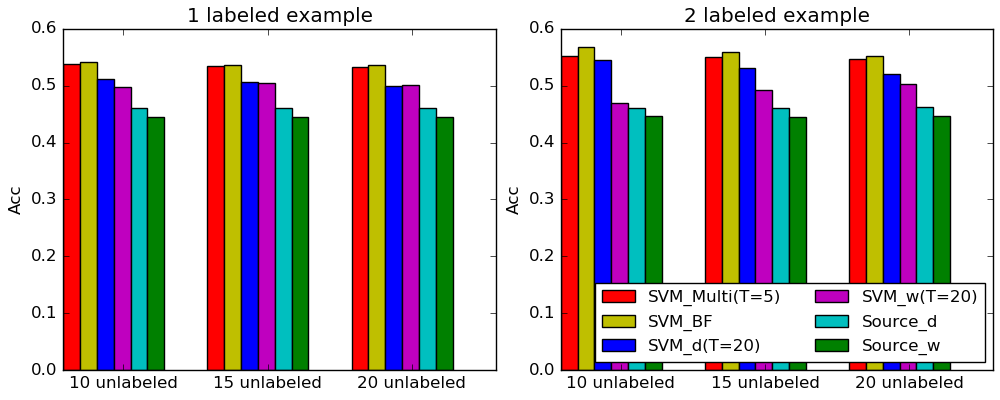
\includegraphics[scale=.50]{aaai/figure/cmp.png}
	\caption{D+W$\rightarrow$A, Multi-source results comparison.}\label{fig:multi}
\end{figure}
\begin{figure}[t]
	\centering
	\begin{tabular}{cccc}
		\subfloat[D $\rightarrow$ A, 10 unlabeled ]{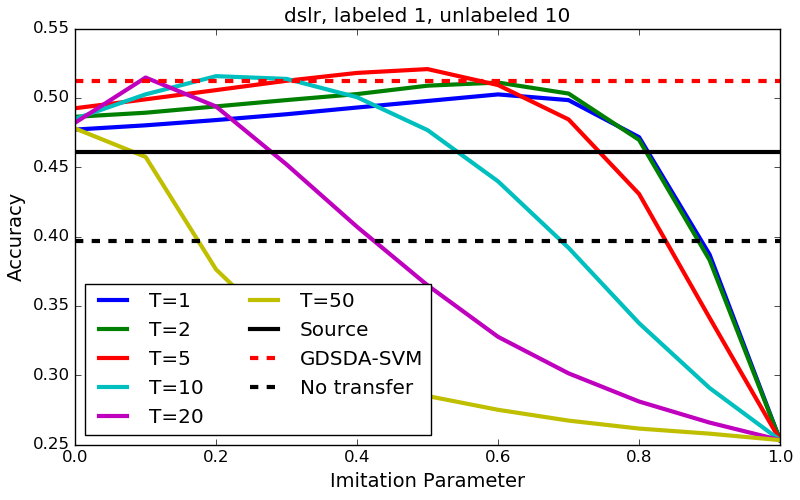
\includegraphics[width=0.45\textwidth]{aaai/figure/dslrtoamazonlabeled1unlabeled10.png}}&
		\subfloat[D $\rightarrow$ A, 15 unlabeled ]{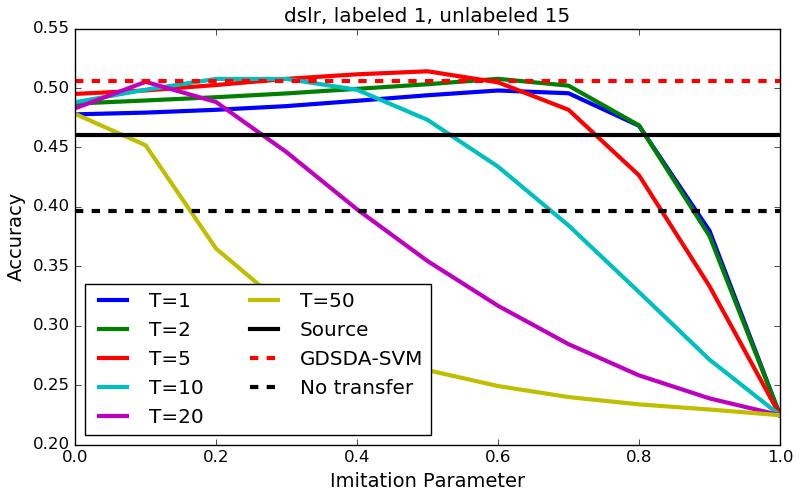
\includegraphics[width=0.45\textwidth]{aaai/figure/dslrtoamazonlabeled1unlabeled15.png}}\\
		\subfloat[D $\rightarrow$ A, 20 unlabeled ]{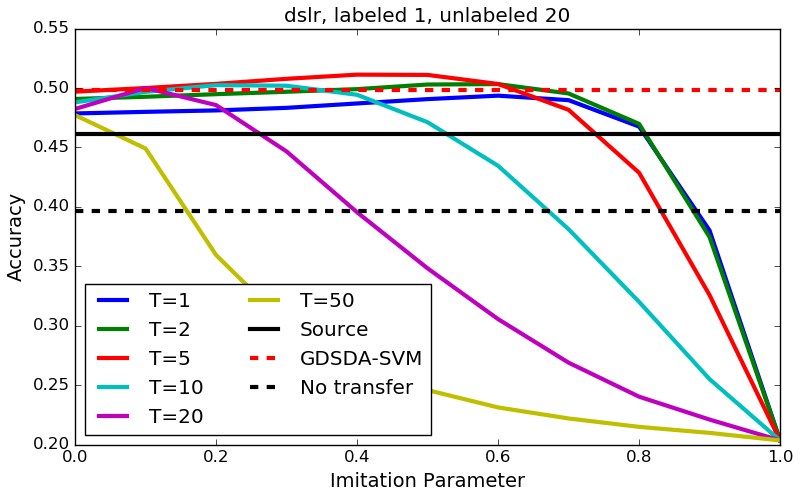
\includegraphics[width=0.45\textwidth]{aaai/figure/dslrtoamazonlabeled1unlabeled20.png}}&
		\subfloat[W $\rightarrow$ A, 10 unlabeled ]{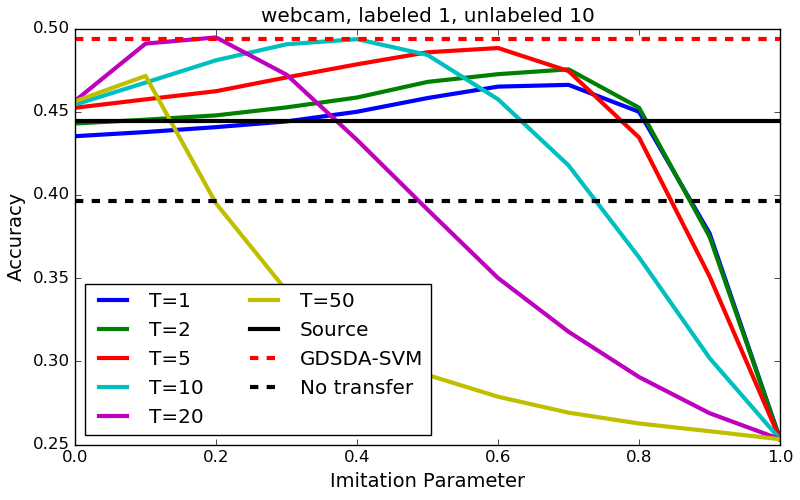
\includegraphics[width=0.45\textwidth]{aaai/figure/webcamtoamazonlabeled1unlabeled10.png}}\\
		\subfloat[W $\rightarrow$ A, 15 unlabeled ]{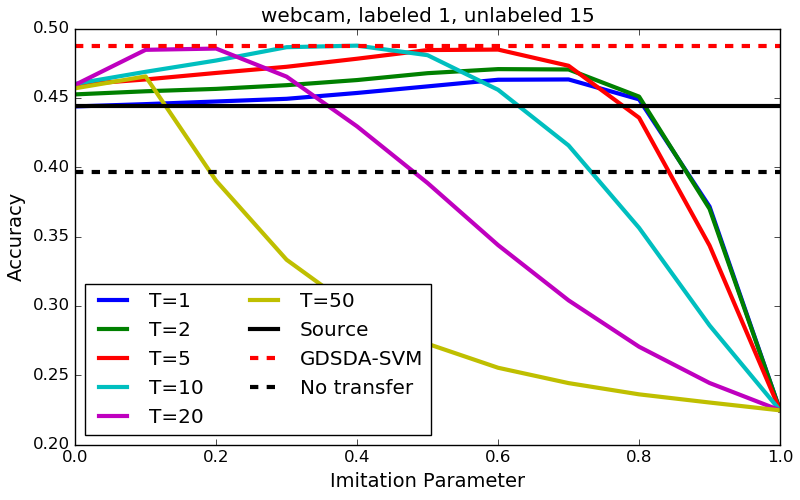
\includegraphics[width=0.45\textwidth]{aaai/figure/webcamtoamazonlabeled1unlabeled15.png}}&
		\subfloat[W $\rightarrow$ A, 20 unlabeled ]{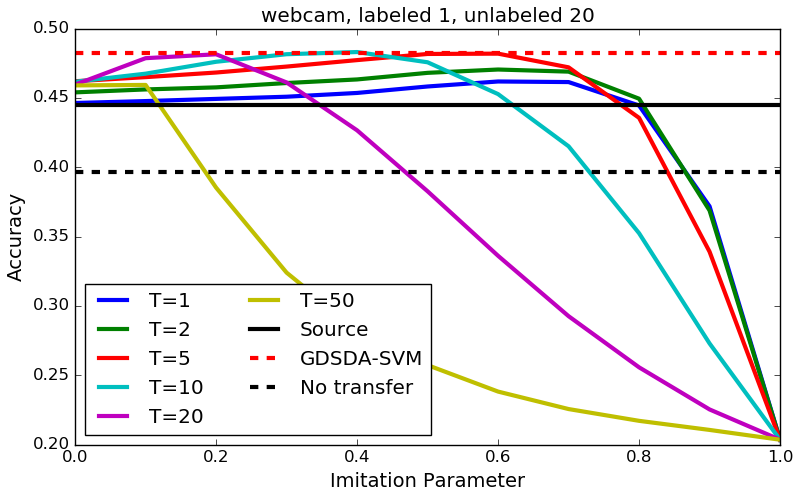
\includegraphics[width=0.45\textwidth]{aaai/figure/webcamtoamazonlabeled1unlabeled20.png}}\\
	\end{tabular}
	\caption{Experiment results on DSLR$\rightarrow$Amazon and Webcam$\rightarrow$Amazon when there are just one labeled examples per class. The X-axis denotes the imitation parameter of the hard label (i.e. $\lambda_1$ in Fig \ref{fig:GDSDA}) and the corresponding imitation parameter of the soft label is set to $1-\lambda_1$.
	}\label{fig:single1}
\end{figure}
Moreover, we can see that GDSDA-SVM can achieve competitive results compared to baselines using brutal force search in D$\rightarrow$A experiments. In W$\rightarrow$A experiments, it achieves the best performances on all 3 different unlabeled sizes. This indicates that we can efficiently (about 6 times faster than the brutal force search) obtain a good target model with GDSDA-SVM.
%\newpage
%\subsubsection{From DSLR to Amazon}


\subsection{Multi-Source for Office datasets}
In this experiment, we show the performance of GDSDA-SVM under the multi-source SDA scenario.
Specifically, we use Amazon as the target domain which can leverage the knowledge of two source models trained from Webcam and DSLR.
We use the similar settings as our single source experiment and perform 2 groups of experiments using 1 labeled and 2 labeled examples per class respectively. We use temperature $T=5$. The results of multi-source GDSDA-SVM are denoted as SVM\_Multi. Here we also include two single source GDSDA-SVMs obtained from the experiments above (SVM\_w and SVM\_d trained using Webcam and DSLR as the source respectively) as the baselines. Moreover, we show the best performance of the brutal force search model (SVM\_BF). For SVM\_BF, we search temperature in range $T=[1,2,5,10,20,50]$ and each imitation parameter in range $[0,0.1,...,1]$. The experiment results are shown in Figure \ref{fig:multi}.

From the results, we can see that, given 2 source models, SVM\_Multi can outperform any single source model trained with GDSDA. This indicates GDSDA-SVM can still exploit the knowledge even in the complex multi-source scenario. Even though SVM\_Multi performs slightly worse than the best result found by brutal force search in some experiments, considering their time consumption (GDSDA-SVM is around 30 times faster than brutal force search), SVM\_Multi still has its advantage in real applications.

\section{Summary}\label{sec:aaai:con}
In this paper, we propose a novel framework called \textit{Generalized Distillation Semi-supervised Domain Adaptation} (GDSDA) that can effectively leverage the knowledge from the source domain for SDA problem without accessing to the source data. To make GDSDA more effective in real applications, we proposed our method called GDSDA-SVM and show that GDSDA-SVM can effectively determine the imitation parameter for GDSDA. 
In our future work, we plan to use a more advanced hyperparameter optimization method, which can optimize the imitation parameter $\lambda$ and the temperature $T$ in GDSDA simultaneously, and expect
further performance improvement 